\scanpage{5}
\mspage{1}

\uline{Courbes} \inserted{exceptionnelles} \uline{de type} $(1,1)$ (sur $\mathbb C$)

A) \uline{Courbe} \inserted{ell.} \uline{anharmonique de type carré}

Cat. de ces courbes équivalente : celle des carrés
\unsure{com}binatoires orientés, i.e. des torseurs sous
\[
\mathbb Z/4\mathbb Z\simeq\mu_4(\mathbb C)\simeq\text{groupe des unités algébriques de }\mathbb Q[i]
\]
\margin{i.e. groupe des unités de $\mathbb Z[i]$ (\unsure{ann}eau des entiers de $\mathbb Q[i]$}

La donnée d'un tel torseur \inserted{$S$} permet de tordre
$\mathbb E\ell_0\overset{\mathrm{def}}\simeq\mathbb C/\mathbb Z[i]$ et trouver
\[
\mathbb E\ell_0(S)\simeq\mathbb E\ell_0\mathbin{\wedge}_{\mathbb Z/4\mathbb Z}S
\]

\margin{\figure{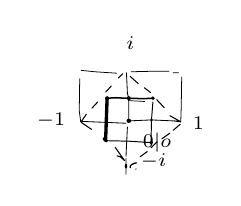
\begin{tikzpicture}[x=.006cm,y=-.006cm,line cap=round,line join=round] \draw[line width=.28pt] (60,72)--(89,75)--(135,78) (166,75)--(207,74)--(246,74) (255,77)--(266,77); \draw[line width=.28pt] (57,90)--(56,158)--(59,180) (273,86)--(272,149)--(271,180); \draw[line width=.38pt] (148,79)--(139,88) (124,105)--(112,118) (95,139)--(83,152) (71,165)--(60,181); \draw[line width=.38pt] (164,85)--(181,100) (194,109)--(207,119) (220,134)--(236,151) (248,168)--(271,181) (256,179)--(271,181); \draw[line width=.38pt] (270,186)--(255,199) (248,205)--(231,217) (221,223)--(208,236) (200,244)--(185,255); \draw[line width=.38pt] (60,182)--(82,197) (132,235)--(152,263) (136,253)--(143,255)--(152,263); \draw[line width=.55pt] (115,131)--(133,130)--(154,131)--(161,131)--(192,132)--(212,131); \draw[line width=.25pt] (160,136)--(195,138); \draw[line width=1.2pt] (115,131)--(113,187)--(112,216)--(109,217)--(113,221); \draw[line width=.35pt] (212,139)--(209,177)--(208,225) (113,221)--(160,222)--(208,225); \draw[line width=.3pt] (156,77)--(158,121)--(161,131)--(161,179) (158,192)--(155,254) (155,259)--(155,292); \draw[line width=.3pt] (59,180)--(155,184) (161,179)--(209,177)--(254,179); \fill (115,131) ellipse[x radius=4.5,y radius=4.2]; \fill (161,131) ellipse[x radius=4.1,y radius=4.5]; \fill (212,131) ellipse[x radius=4.1,y radius=4.1]; \fill (161,179) ellipse[x radius=5.0,y radius=4.5]; \fill (209,174)--(212,177)--(209,181)--(206,177)--cycle; \fill (113,221) ellipse[x radius=3.8,y radius=4.0]; \fill (208,225) ellipse[x radius=4.2,y radius=3.9]; \fill (155,275) ellipse[x radius=2.7,y radius=5.0]; \node[font=\scriptsize,anchor=east] at (47,179) {$-1$}; \node[font=\scriptsize,anchor=west] at (276,183) {$1$}; \node[font=\scriptsize,anchor=south] at (164,49) {$i$}; \node[font=\scriptsize,anchor=north west] at (170,184) {$\unsure{0|o}$}; \node[font=\scriptsize,anchor=west] at (166,264) {$-i$}; \draw[line width=.48pt] (177,268) .. controls (170,269) and (162,273) .. (164,278); \fill (176,281) circle[radius=1.4]; \end{tikzpicture}}}

Si le carré est réalisé comme carré \inserted{euclidien}
dans un plan euclidien \inserted{$V_S$} (canoniquement), de centre $\unsure{0|o}$,
\figure{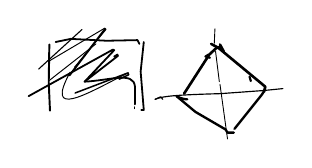
\begin{tikzpicture}[x=.008cm,y=-.008cm,line cap=round,line join=round] \draw[line width=.7pt] (40,34)--(39,94)--(41,139); \draw[line width=.65pt] (50,30)--(74,25)--(131,28)--(180,27)--(183,33); \draw[line width=.65pt] (190,30)--(185,77)--(190,138)--(186,138); \draw[line width=.4pt] (23,73)--(92,10); \draw[line width=.35pt] (40,60)--(128,8)--(130,10)--(80,70); \draw[line width=.7pt] (128,10)--(72,83); \draw[line width=.35pt] (40,91)--(114,33); \draw[line width=.65pt] (7,116)--(141,42)--(143,43)--(96,93)--(149,52)--(148,50)--(143,53); \draw[line width=.35pt] (73,78) .. controls (32,153) and (98,113) .. (161,81); \draw[line width=.55pt] (81,111)--(165,79)--(166,82)--(151,89); \draw[line width=.65pt] (96,93) .. controls (137,91) and (174,76) .. (176,101) -- (176,129); \draw[line width=.35pt] (175,133)--(175,136); \begin{scope}[shift={(200,5)}] \draw[line width=.32pt] (103,4)--(102,27) (104,40)--(110,88) (111,92)--(123,179); \draw[line width=.42pt] (8,116) .. controls (20,111) and (40,109) .. (112,107) -- (181,102)--(211,99); \draw[line width=.42pt] (8,116)--(17,112)--(20,116); \draw[line width=.95pt] (54,107)--(94,45)--(107,33) (107,33)--(183,96)--(181,104); \draw[line width=.95pt] (97,28)--(108,34) (111,29)--(117,40)--(108,33); \draw[line width=.8pt] (93,45)--(88,48)--(95,50) (158,80)--(160,87); \draw[line width=.85pt] (42,111) .. controls (49,115) and (55,116) .. (59,116); \draw[line width=.85pt] (42,111)--(72,136)--(120,164)--(123,169)--(133,169); \draw[line width=.85pt] (134,163)--(178,108)--(181,103); \end{scope} \end{tikzpicture}}
on en déduit dans le plan (vectoriel via $\unsure{0|o}$) $V_S$
un syst. de deux \deleted{\unsure{axes} de}
coordonnées \inserted{mod. signes\unsure{,}}
via les diagonales, d'où un
\deleted{\unsure{lattice}} \inserted{réseau}
$\Gamma_S$ dans $V_S$ (sous-groupe discret de
rang $2$) et
\begingroup \setbox0=\hbox{$\displaystyle \mathbb E\unsure{\ell_0(S)\,2|\ell_0(S)/2}X_S=V_S/\Gamma_{\unsure{r|\Gamma|S}}.$} \[ \rlap{\begin{tikzpicture}[overlay,x=\wd0,y=1ex,line cap=round,line join=round] \draw[line width=.35pt] (-.43,-1.0) .. controls (-.27,-1.3) and (-.08,-.9) .. (-.055,-.5) .. controls (-.05,.25) and (-.08,1.4) .. (-.10,2.1) -- (.45,2.0) -- (1.04,2.4) -- (1.07,-.7) -- (1.18,-.65); \end{tikzpicture}} \copy0 \] \endgroup

\margin{\figure{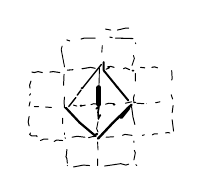
\begin{tikzpicture}[x=.006cm,y=-.006cm,line cap=round,line join=round] \draw[line width=.35pt] (182,14)--(193,16) (207,16)--(224,12)--(231,12); \draw[line width=.38pt] (100,37)--(106,39) (130,35)--(137,33)--(160,33) (191,31)--(196,32) (203,33)--(240,34); \draw[line width=.32pt] (90,50)--(88,57)--(95,94) (175,49)--(174,63) (245,43)--(246,45) (241,70)--(243,76)--(238,91); \draw[line width=.38pt] (26,105)--(31,106)--(39,104)--(48,106) (64,105)--(71,104)--(85,106) (101,101)--(113,100) (132,98)--(150,95)--(160,97); \draw[line width=.38pt] (183,99)--(190,96) (186,94)--(193,93)--(200,95) (220,98)--(224,96)--(233,100) (256,95)--(265,96) (280,95)--(286,94)--(292,96); \draw[line width=.35pt] (322,102)--(323,119)--(322,122) (321,153)--(324,162) (325,176)--(323,191) (323,206)--(326,230); \draw[line width=.35pt] (24,124)--(21,133)--(22,139) (23,151)--(21,154) (22,168)--(20,177) (20,199)--(18,211)--(20,219) (23,234)--(21,237)--(25,240)--(36,240); \draw[line width=.35pt] (94,110)--(93,133) (95,158)--(94,168)--(95,181) (91,203)--(91,214) (95,234)--(95,237) (96,244)--(97,245) (100,269)--(99,281)--(98,284)--(100,288)--(101,298); \fill (101,303) circle[radius=1.2]; \draw[line width=.35pt] (245,108)--(245,124) (243,153)--(241,160)--(242,170)--(246,169) (237,178)--(240,200)--(244,216) (242,251)--(242,254) (243,271)--(245,276)--(242,291) (246,301)--(248,303); \draw[line width=.35pt] (31,178)--(40,178) (55,179)--(67,180) (114,175)--(121,177) (129,177)--(139,175) (151,174)--(157,172)--(164,173); \draw[line width=.35pt] (182,173)--(189,171)--(200,172) (224,171)--(237,168) (248,171)--(263,172) (288,170)--(297,168); \fill (269,172) circle[radius=.7]; \draw[line width=.35pt] (37,242)--(36,240) (44,250)--(51,247)--(60,247) (73,252)--(78,249)--(91,250) (111,243)--(122,241)--(138,243) (146,244)--(153,242)--(162,241); \draw[line width=.35pt] (183,243)--(199,242) (218,239)--(223,237)--(238,239) (260,239)--(264,238) (281,238)--(285,236)--(292,236) (309,234)--(314,233)--(318,234); \draw[line width=.35pt] (114,306)--(135,302)--(148,303) (180,304)--(194,302)--(214,299)--(225,302)--(231,300); \draw[line width=.32pt] (169,97)--(168,134) (166,210)--(163,225)--(166,232) (165,253)--(166,270) (165,289)--(165,303); \draw[line width=.5pt] (173,89)--(133,139) (130,143)--(122,154) (119,159)--(104,178); \draw[line width=.7pt] (178,84)--(178,101)--(180,105) (180,104)--(206,136)--(230,165); \draw[line width=.8pt] (98,181)--(127,212)--(159,239)--(164,236); \draw[line width=.85pt] (237,174)--(197,213)--(166,246); \draw[line width=1.25pt] (231,181)--(215,201); \draw[line width=1.8pt] (168,138)--(168,173); \draw[line width=.6pt] (168,178)--(166,190)--(167,204) (162,183)--(166,179) (171,196)--(168,201); \foreach \x/\y in {132/139,206/136,127/212,197/213,169/173,130/176,200/174,240/102}{\fill (\x,\y) ellipse[x radius=3.1,y radius=2.3];} \fill (167,204) circle[radius=1.6]; \end{tikzpicture}}}

Il y a dans $X_S$ un élement\raisebox{-.6em}{\unsure{:}} d'ordre $2$ canonique
\inserted{$\eta_S$}
(stable par automorphismes), les deux autres él. d'
ordre $2$ sont échangés par le générateur $i$ de
$\mu_4(\mathbb C)\simeq\operatorname{Aut}(\unsure{X_S|X})$.
(\leavevmode\hbox{\rlap{\kern.30em\underline{\kern-.30em\phantom{NB}}}NB} $\eta_S$ \unsure{peu}t donc être \unsure{défini}

\margin{4}
